\section{Analysis of thermal conditions along the mission}
\label{sec:TCS_phases}

In this section, the mission will be analyzed and divided in perspective of thermal environment encountered. During this study, the internal heat flux generated by instrumentation won't enter the reasoning.
This is done because its maximum value and its variability are both contained during the mission, so it won't affect the sectioning of the TPs and the selection of the hot and the cold cases.
The architecture of the S/C won't affect the reasoning and only the heat fluxes from the external environment (Sun flux, planets' albedo and IR emission) will enter this preliminary analysis. A deeper study will be conducted during the reverse sizing in \autoref{sec:TCS_sizing}.

\subsection{Thermal phases analysis}
\label{subsec:TP_analysis}

Different thermal conditions have been encountered by Juno during its cruise. In previous chapters, the mission was divided into phases by different attitude and communication constraints.
These phases will be now grouped by the means of thermal constraints to better analyze their evolution during the mission time.

\begin{itemize}
    \item \textbf{TP-1}:
    in this first phase, which comprehends both LEOP and IC-1, the S/C is in SPM due to thermal and power requirements. In particular, since the trajectory is relatively close to the Sun, Juno has to protect the vault with the HGA (as already explained in the previous chapters).
    Even if TP-1 is considered a hot phase, it is not the most critical as other phases have more stringent requirements, facing longer periods closer to external heat sources (i.e. Sun and Earth).

    \item \textbf{TP-2}:
    this second phase corresponds to IC-2. Among the ICs it is the longest and the only one featuring EPM. It does not call for any particular thermal requirement, being Juno farther from both Sun and Earth.
    No specific attitude is required to thermally control the S/C during the different manoeuvres performed during IC-2. Neither hot nor cold phase is considered along TP-2.
    
    \item \textbf{TP-3}:
    the third thermal phase consists of IC-3 till the EGA, performed in SPM to protect the electronics inside the vault as the S/C passes through the perihelion of the orbit (at 0.88 AU).
    During TP-3, Juno was found to face the most relevant hot environment, occurring at the closest approach to the Sun. As a consequence, this condition was selected to be the hot case.
    
    \item \textbf{TP-4}:
    the fourth phase analyzed consists only of the EGA, from the entrance till the exit of Juno from Earth's SOI. This phase contains both a possible hot case and a possible cold case, the first due to the proximity to the planet, the latter due to the eclipse.
    As a consequence, this is the phase when Juno faces the highest flux excursion of the entire mission.
    It was found that both of the two conditions are the most extreme in terms of heat flux as the obtained results are linked with the simplified model used.
    As explained in \autoref{subsec:heat_flux_analysis}, these conditions won't be selected as hot or cold case.

    \item \textbf{TP-5}:
    this phase is the continuation of the TP-3, except that the S/C does not encounter such high flux environment as at perihelion. It goes from the end of EGA till the end of IC-3.
    
    \item \textbf{TP-6}:
    this phase only includes the OC up to JOI. The S/C encounters a progressively colder environment as it is going away from the Sun.
    However, knowing its trajectory, Juno will face colder contexts along its mission. The transition between TP-6 and TP-7 can be seen in \autoref{fig:Jupiter_flux_analysis_ext}.

    \item \textbf{TP-7}:
    the last phase goes from the JOI till the end of the mission, including all the science orbits around Jupiter.
    During this period of time, the spacecraft is subject to the harsh environment of Jupiter, where it faces oscillating flux from the planet: higher nearby the perijoves and lower at the apojoves.
    Overall, the environment stays cold during the whole phase with a minimum when both Jupiter and Juno are around the apocentre of their respective orbits. This condition is elected as the coldest case of the entire mission.
    
\end{itemize}


\subsection{External heat flux analysis}
\label{subsec:heat_flux_analysis}

In order to find the hot and the cold cases, a simplified model of the main external heat fluxes has been carried out. All the formulas for this analysis are reported in \autoref{sec:TCS_sizing}.
To facilitate the computation, some assumptions have been adopted:
\vspace*{2mm}
\begin{itemize}
    \item as previously mentioned, only the external heat fluxes have been modeled discarding the internal contribution, which is better treated in \autoref{sec:TCS_sizing};
    \item the only contribution considered during the interplanetary phases is the Sun flux, while in proximity of the planets also albedo and IR emissions are added;
    \item for the hot case only TP-3 and TP-4 have been analyzed, since the other phases do not have critical condition in this sense;
    \item for the cold case TP-4, TP-6 and TP-7 have been analyzed, the first because of the criticality of the eclipse condition, the second because of the increasingly farther position of the S/C with respect to the Sun in an interplanetary environment, the third because Juno is orbiting Jupiter at its farthest points from the Sun;
    \item the analysis has been carried out from the ephemeris of the real mission instead of taking the nominal cruise;
    \item the $\cos \theta$ factor in the albedo formula is assumed to be always equal to $1$ as a conservative simplification, so only the distances are taken into account during the calculations.

\end{itemize}

The external heat fluxes computed by this simplified model for TP-3 (\autoref{fig:Perihelion_flux_analysis}), transition between TP-6 and TP-7 (\autoref{fig:Jupiter_flux_analysis_ext}) and TP-4 (\autoref{fig:EGA_flux_analysis}) are shown in the plots below.

\twofig{Perihelion_flux_analysis}{Flux analysis of TP-3}
    {Jupiter_flux_analysis_ext}{Flux analysis of TP-7}{1}

\begin{minipage}{0.5\linewidth}
    \centering
    \captionsetup{type=figure}
    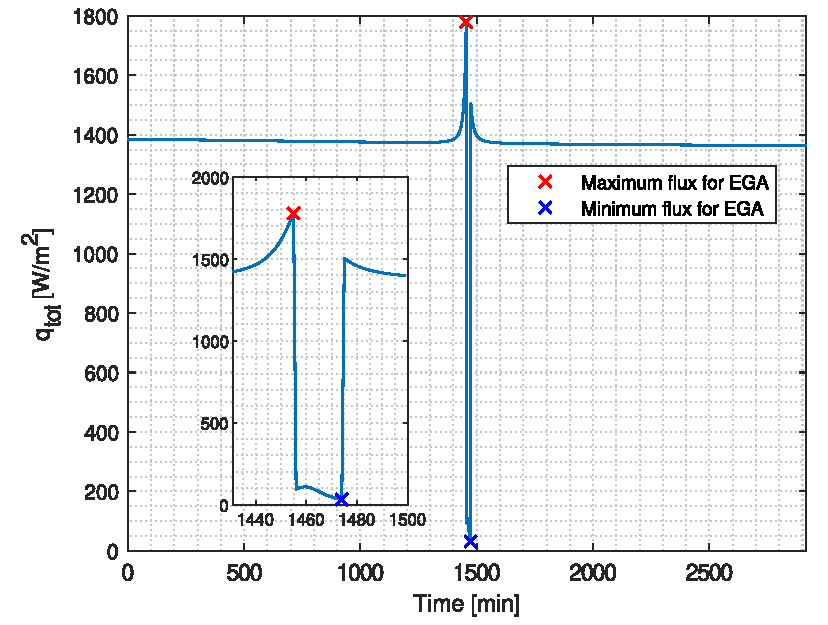
\includegraphics[width=\linewidth]{Images/EGA_flux_analysis.pdf}
    \caption{Flux analysis of TP-4 (EGA phase)}
    \label{fig:EGA_flux_analysis}
\end{minipage}\hfill
\begin{minipage}{0.5\linewidth}
    \centering
    \captionsetup{type=table}
    \renewcommand{\arraystretch}{1.4}
    \begin{tabular}{|c|c|}
        \hline
        \textbf{Phase} &
        \textbf{Total heat flux [$\boldsymbol{\textbf{W/m}^2}$]} \\
        \hline
        \hline
        \textbf{TP-4 hot case}      & 1779.32   \\
        \hline
        \textbf{TP-3 hot case}      & 1759.23   \\
        \hline
        \hline
        \textbf{TP-4 cold case}     & 31.13     \\
        \hline
        \textbf{TP-7 cold case}     & 45.62     \\
        \hline
    \end{tabular}
    \caption{Summary of considered hot and cold cases}
    \label{table:cases}
\end{minipage}

\vspace*{4mm}

It is worth noting that the flux derived from both planets' albedo contribution is greatly overestimated due to the simplification discussed before.
Despite TP-4 presents both the hottest and the coldest points of the whole mission, the time spent by Juno in these regions is limited.
As can be noticed in \autoref{fig:EGA_flux_analysis}, the S/C spends only around half a minute in an environment characterized by a heat flux above the one of the hot case (TP-3) and spends around four minutes in an environment where the heat flux is below the one of the cold case (TP-7).
Moreover, as can be also seen in \autoref{table:cases}, the cases are very close to each other.
For this reason, the choice is to not consider EGA's peaks as hot and cold cases, also because in reality Juno has to overcome a transient before reaching extreme temperatures.
The passage from perihelion during TP-3 is hence selected to be the most significant hot environment.
On the other side, the most relevant cold case was found to be a few orbits after JOI, around the farthest position of Juno from both Sun and Jupiter, where both solar flux and the planet's contribution are at their lowest.
Particularly, in \autoref{fig:Jupiter_flux_analysis_ext} oscillations with two different frequencies can be observed: the long period one is related to Jupiter's lightly elliptical orbit around the Sun, the short term oscillation, with its peaks, is related to Juno's highly elliptical orbit around Jupiter.
The chosen resolution for the ephemeris determines the non-uniformity of the observed peaks.